

\subsection*{Predicting CO\textsubscript{2} Emissions 2020}
%todo: summarize

In order to predict the emissions for each country for the two next years starting from 2018 we need a model that describes the \co emissions evolution. A model based on regression learning is used.

For choosing the size $k$ of a polynomial $\sum_{n=1}^{k}{a_n*x^n}$, fifteen models of size $k=[1,\dots,15]$ were trained and the results were compared to the real data using the root-mean-sqaure (RMS) in \autoref{fig:RMS}.
\begin{figure}[h!]
	\centering
	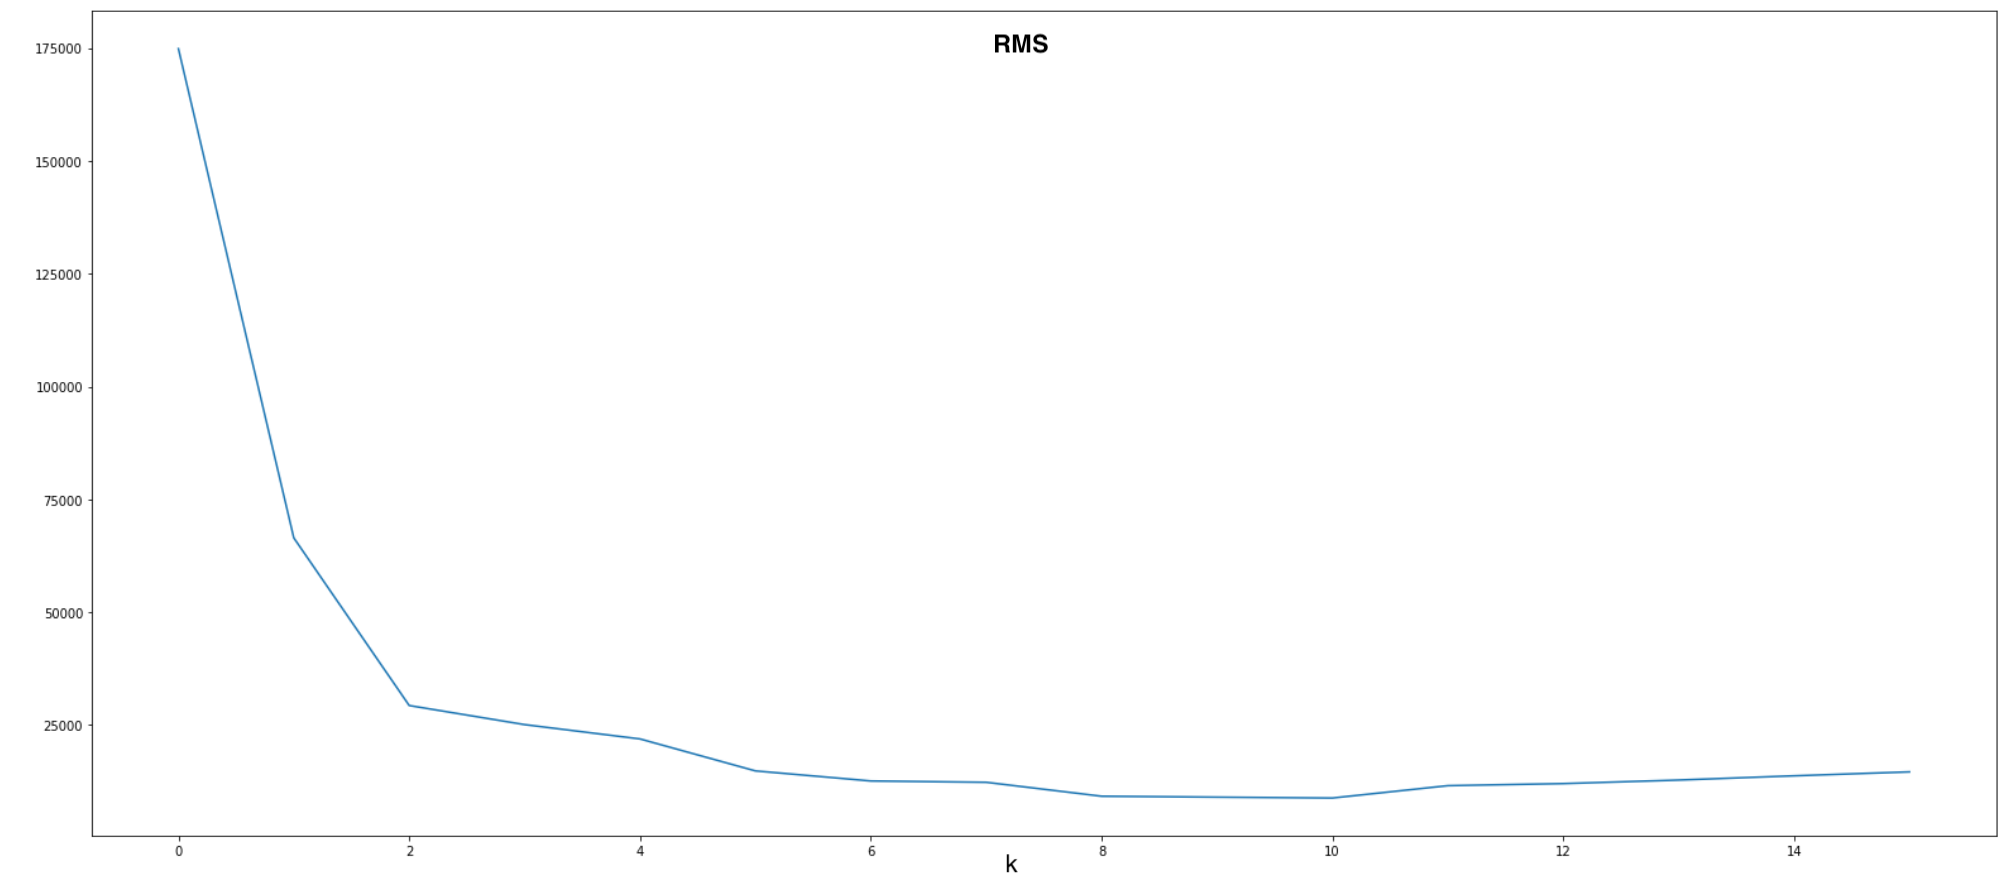
\includegraphics[width=0.7\linewidth]{ziedPNGS/RMS}
	\caption{$k=9$ delivers the smallest error.}
	\label{fig:RMS}
\end{figure}%todo: better plot from Max

%*{Polynomial regression's limitations}
After training a regression model for each country, the polynomials showed some plausible predictions but also many predictions where the curve has a steep drop for 2019 and 2020 \autoref{fig:firstPrediction}. 

%*{Correlation's predictions}
Looking closer to the EDGAR dataset, we can notice that some countries emissions are correlating. This make sense since the industry and a more ressource-intensive way of life becomes more and more global. Using this assumption, one can take advantage of these correlations to correct the wrong predictions from our models.
For each correlation, we train a linear model using the real data from 1970 until 2018 and predict the emissions of 2019 and 2020 using the appropriate model and the predicted data from 1970 to 2020.

%{Results and conclusion}
From the eight major countries we consider -- Canada, China, United States, Japan, Russia, Brazil, India and the EU -- India's predictions could be generated with the first prediction and the remaining countries were generated with the second predictions.
Only Russia's predictions are not available, because no correlation with any other country was found.

\begin{figure}[hbt!]
	\centering
	\subfloat[Brazil]{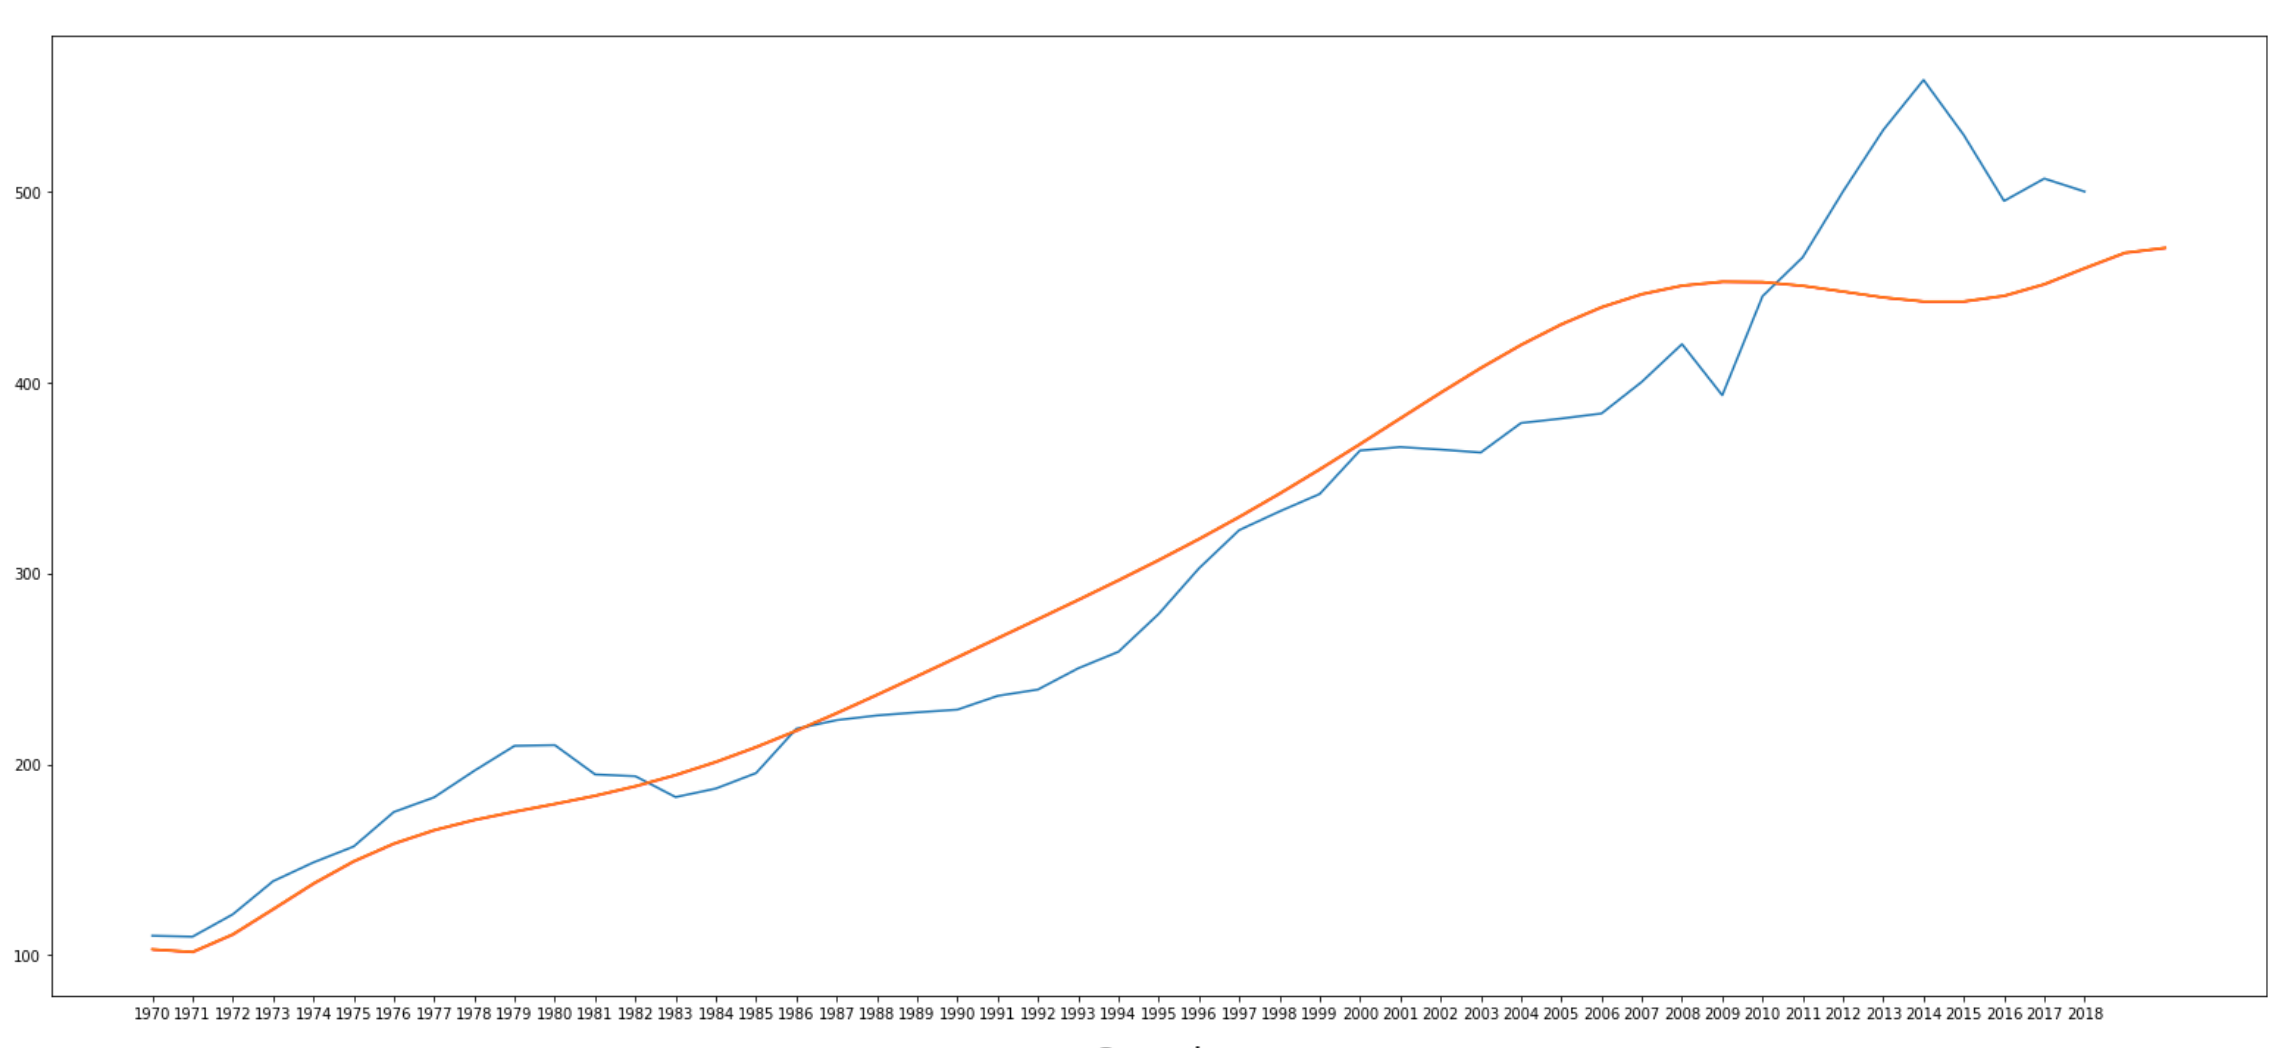
\includegraphics[width=0.5\linewidth]{ziedPNGS/br}}
	\subfloat[Canada]{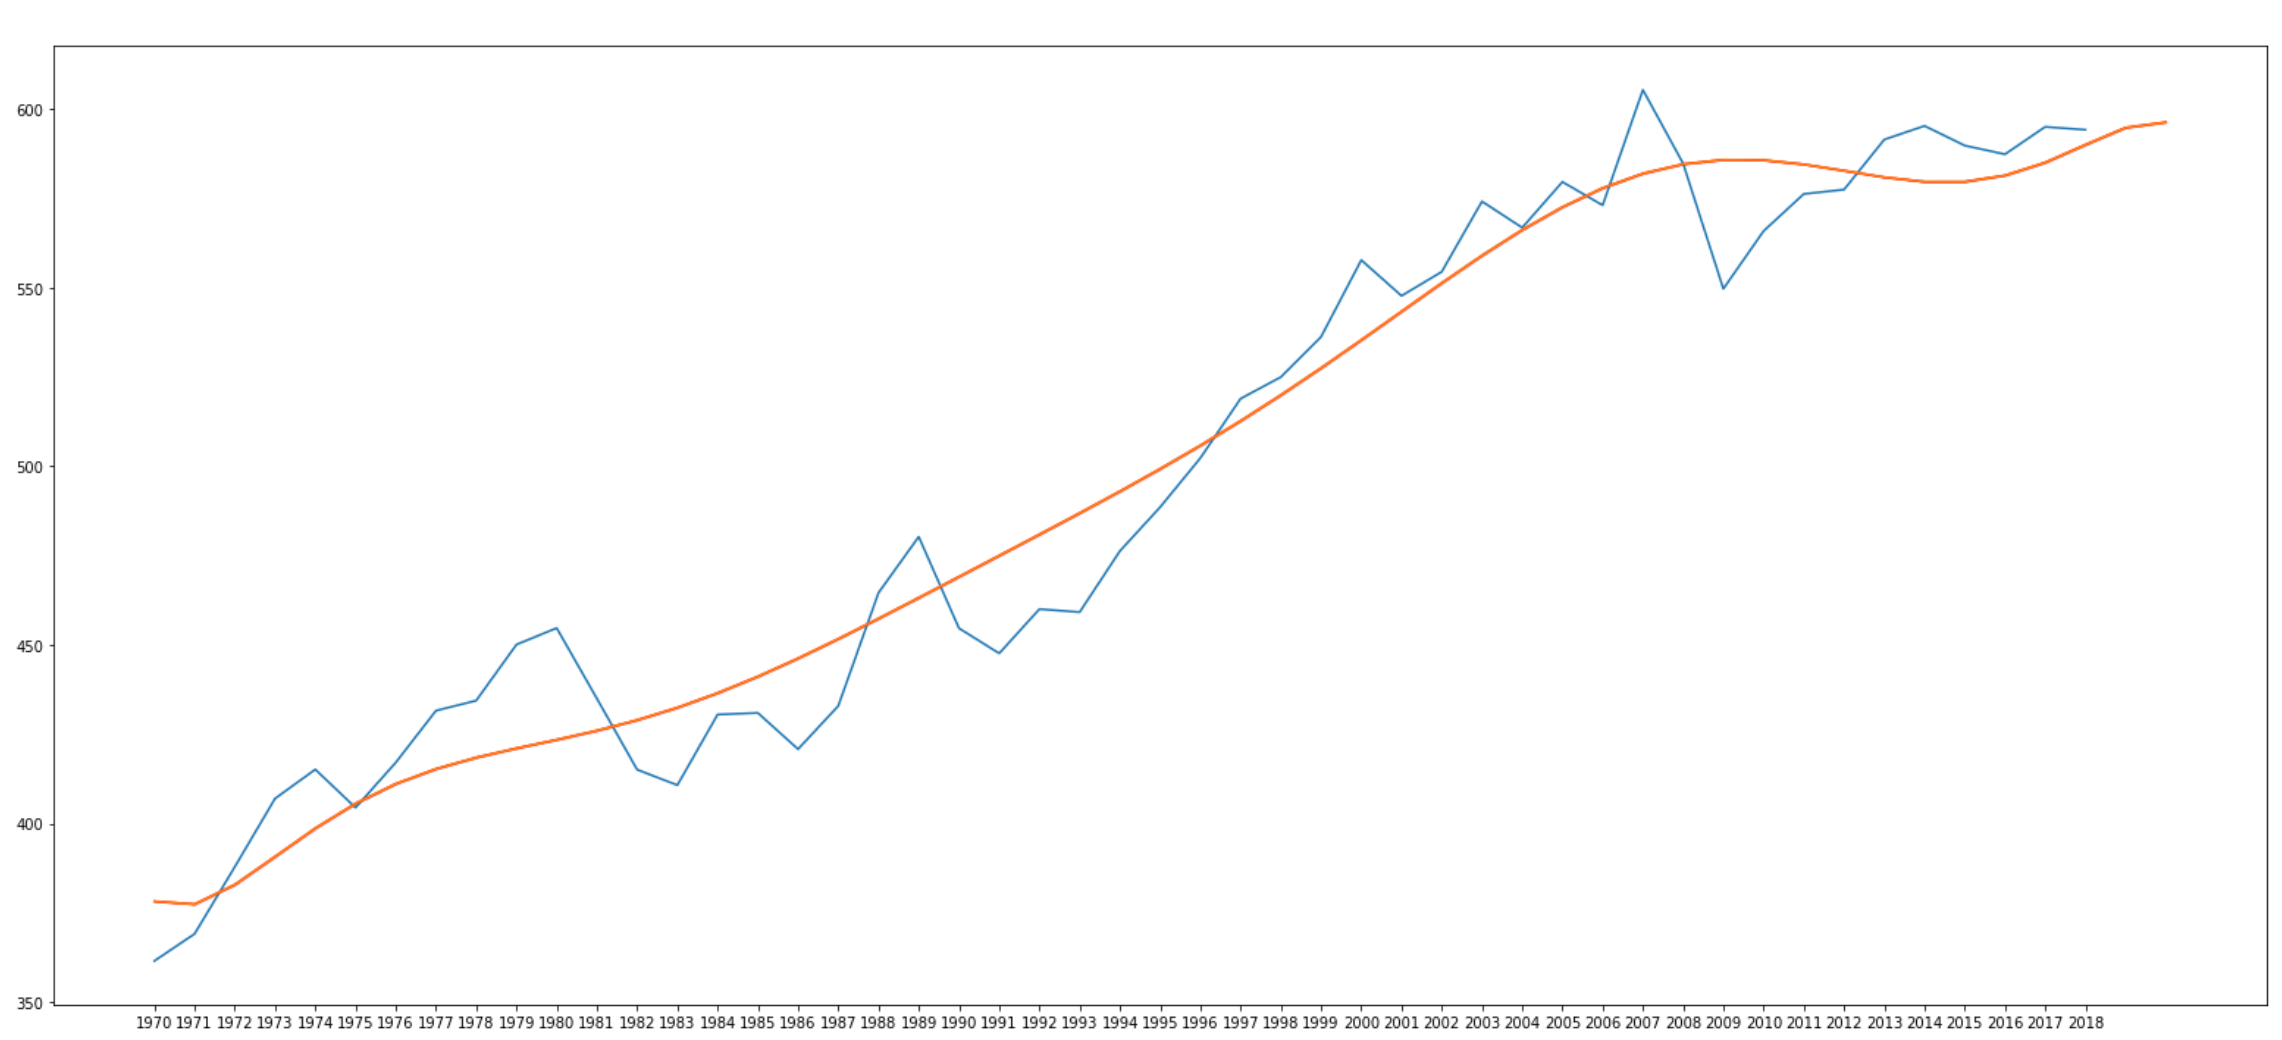
\includegraphics[width=0.5\linewidth]{ziedPNGS/2}}
	
	\subfloat[Japan]{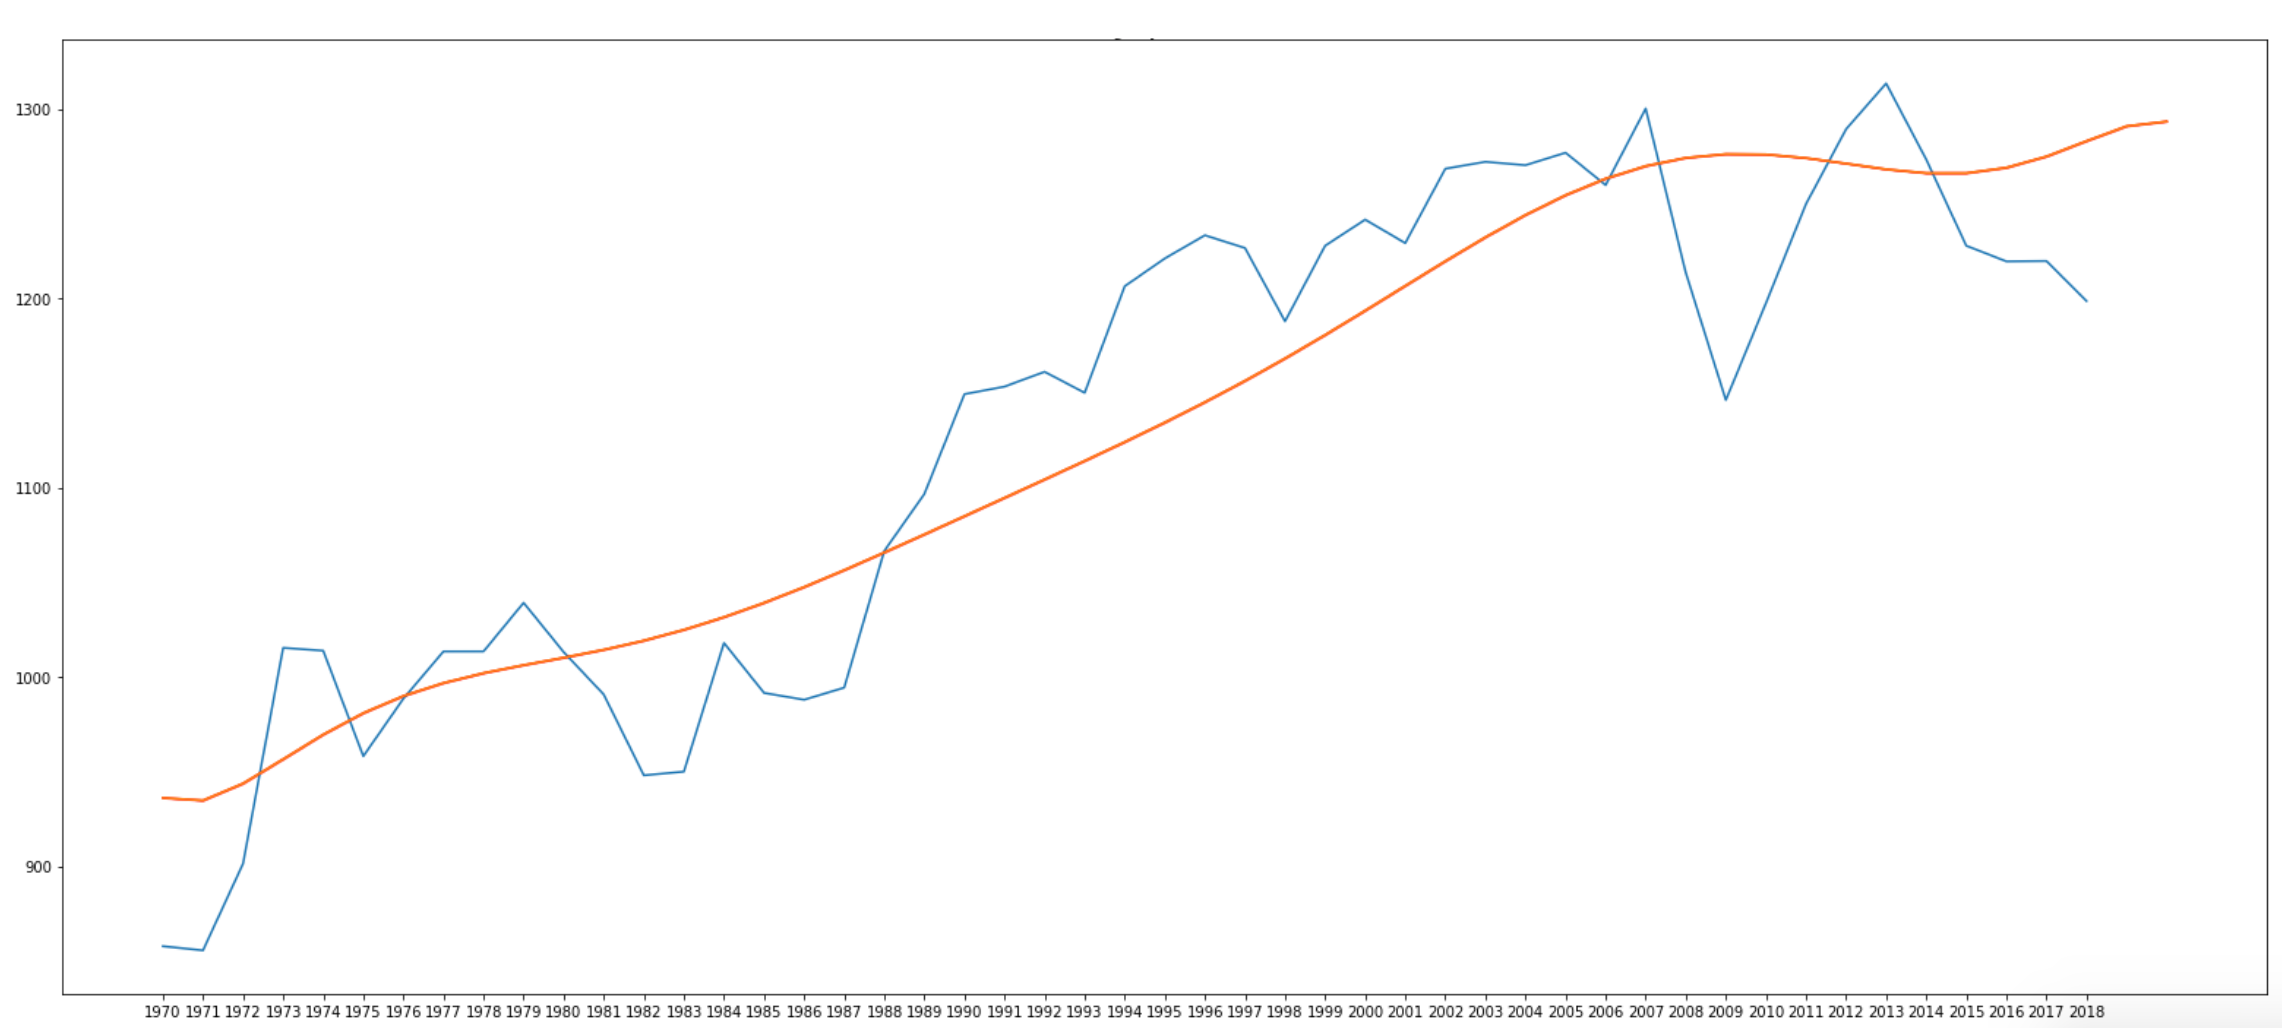
\includegraphics[width=0.5\linewidth]{ziedPNGS/3}}
	\subfloat[China]{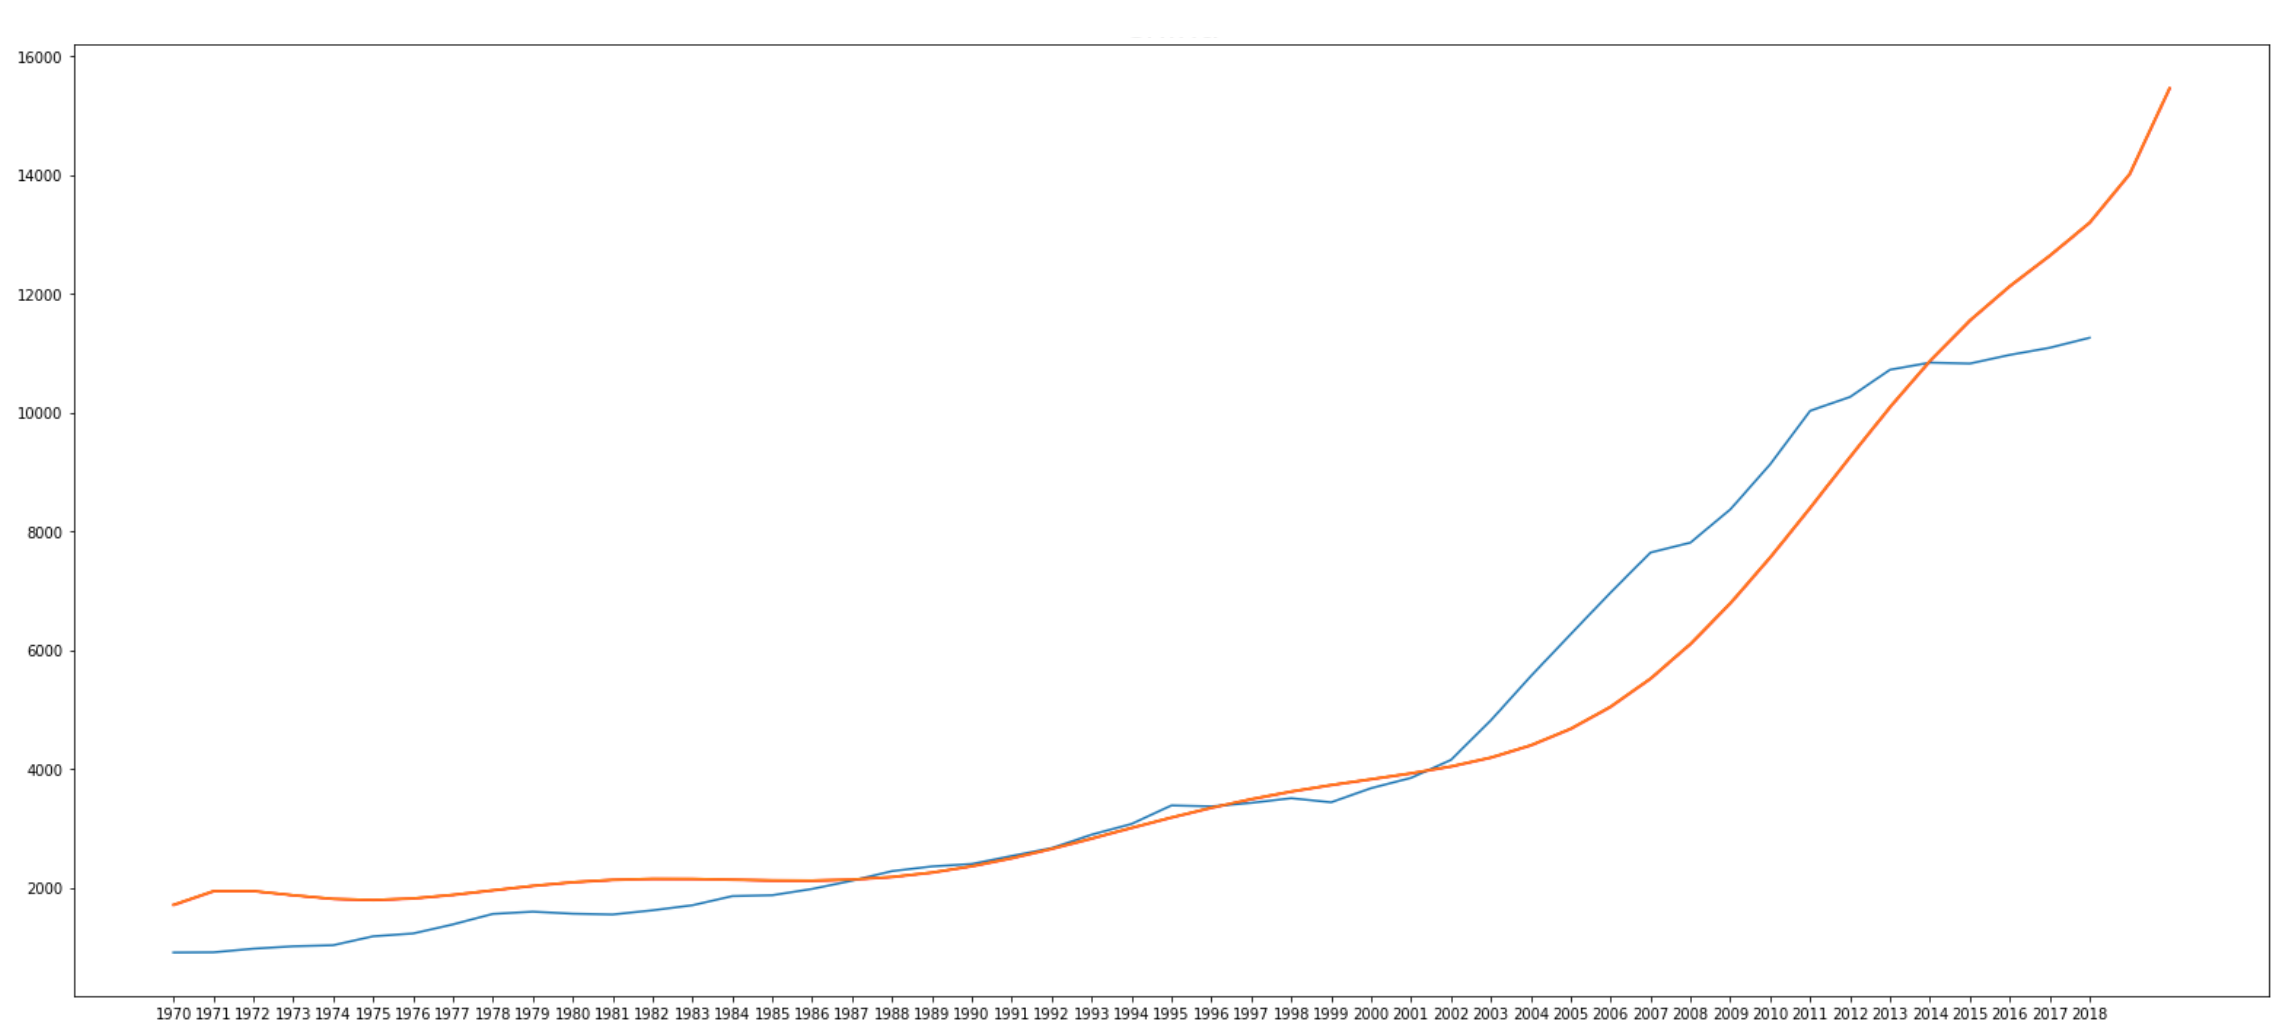
\includegraphics[width=0.5\linewidth]{ziedPNGS/4}}
	
	\subfloat[EU]{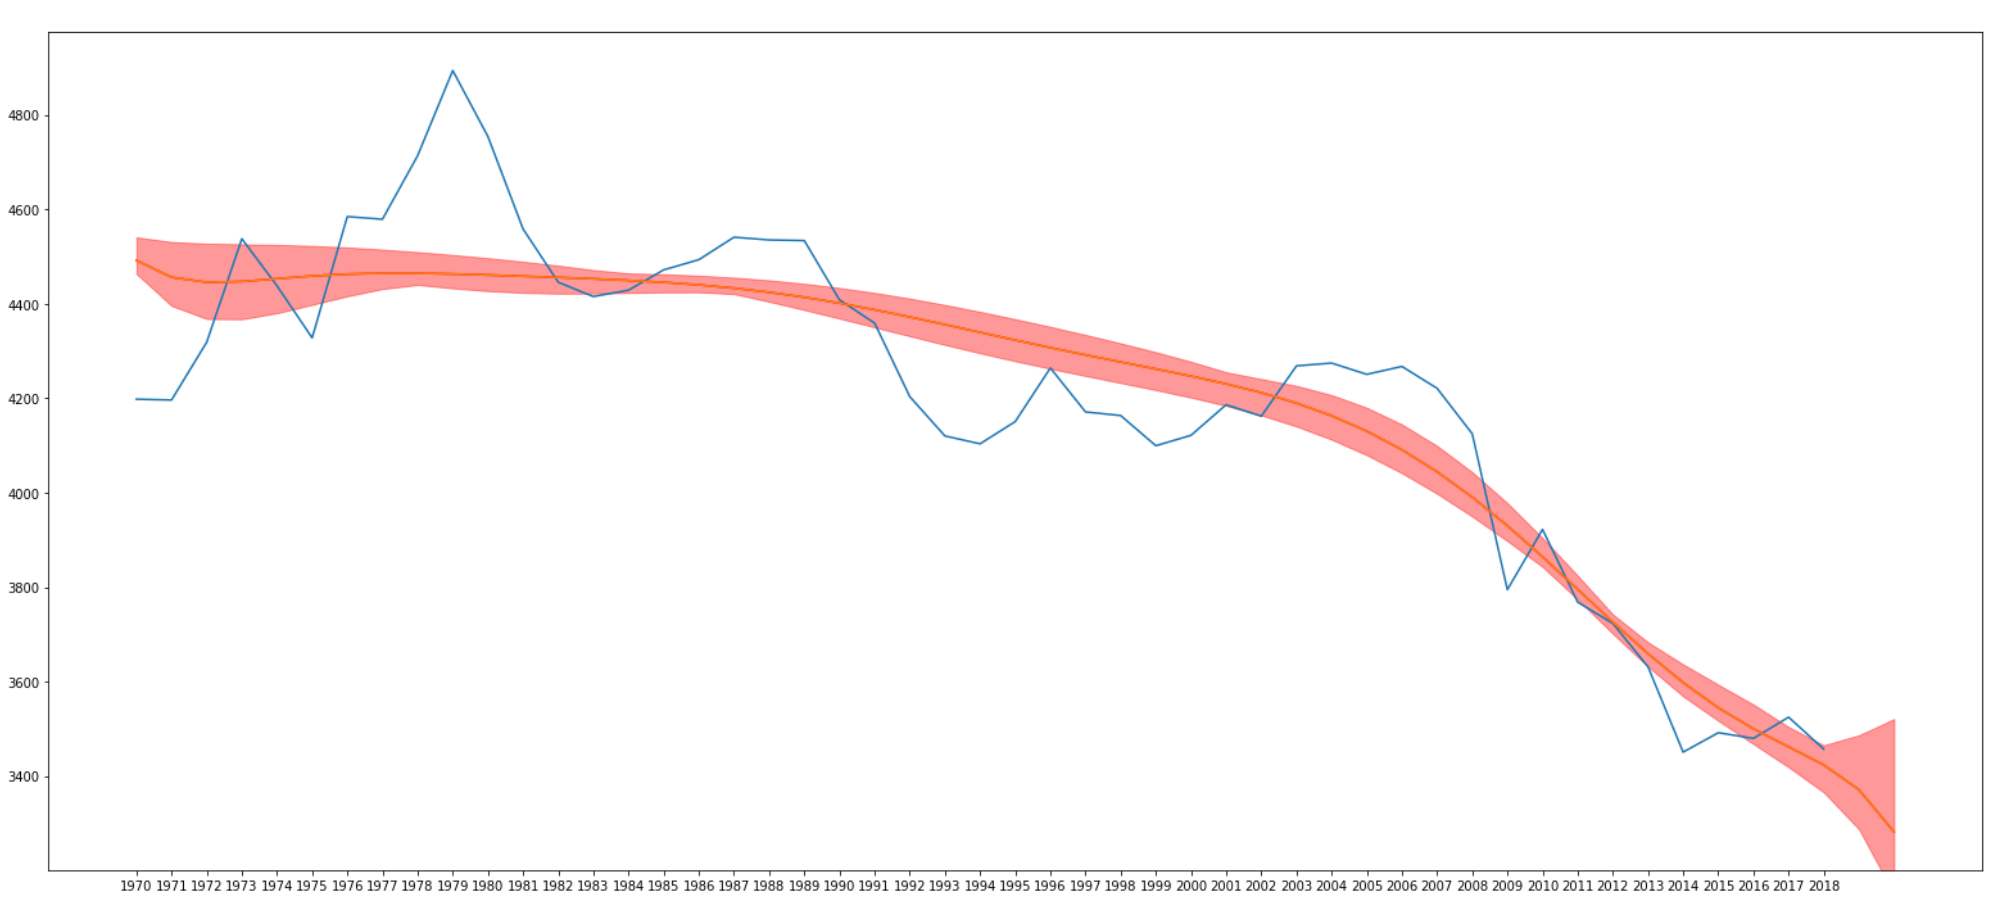
\includegraphics[width=0.5\linewidth]{ziedPNGS/5}}
	\subfloat[United States]{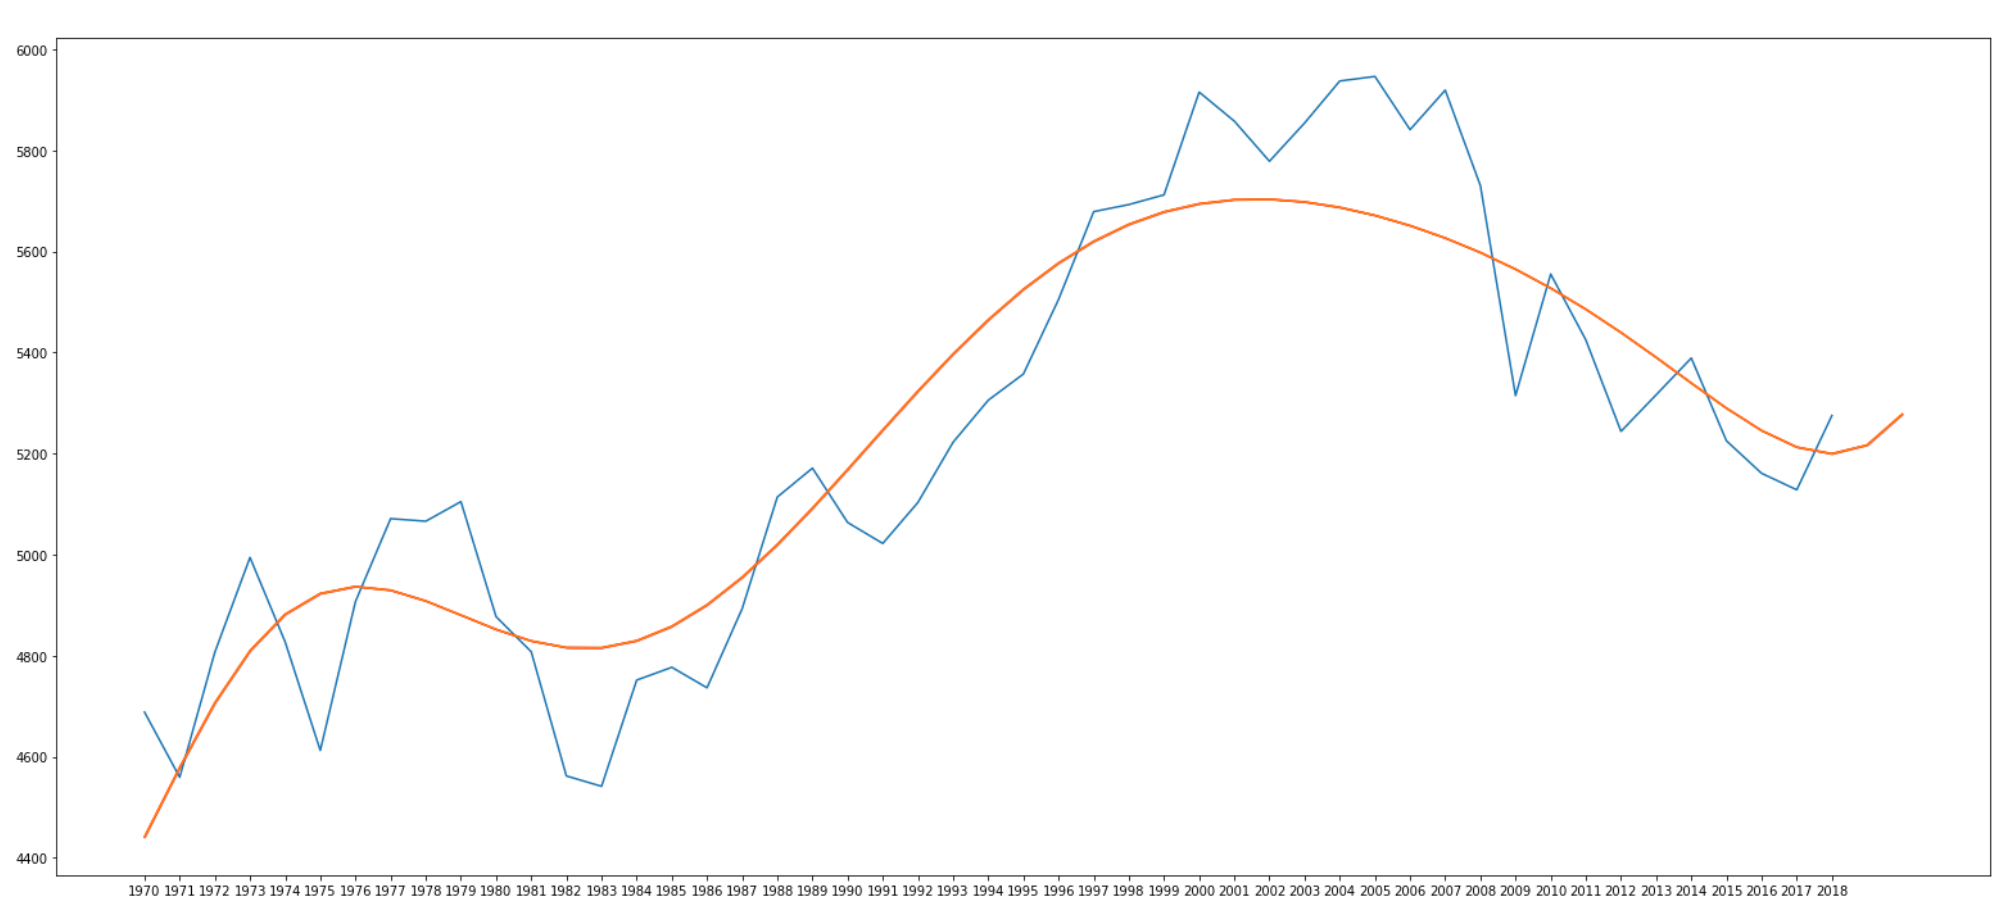
\includegraphics[width=0.5\linewidth]{ziedPNGS/6}}
	
	\subfloat[India]{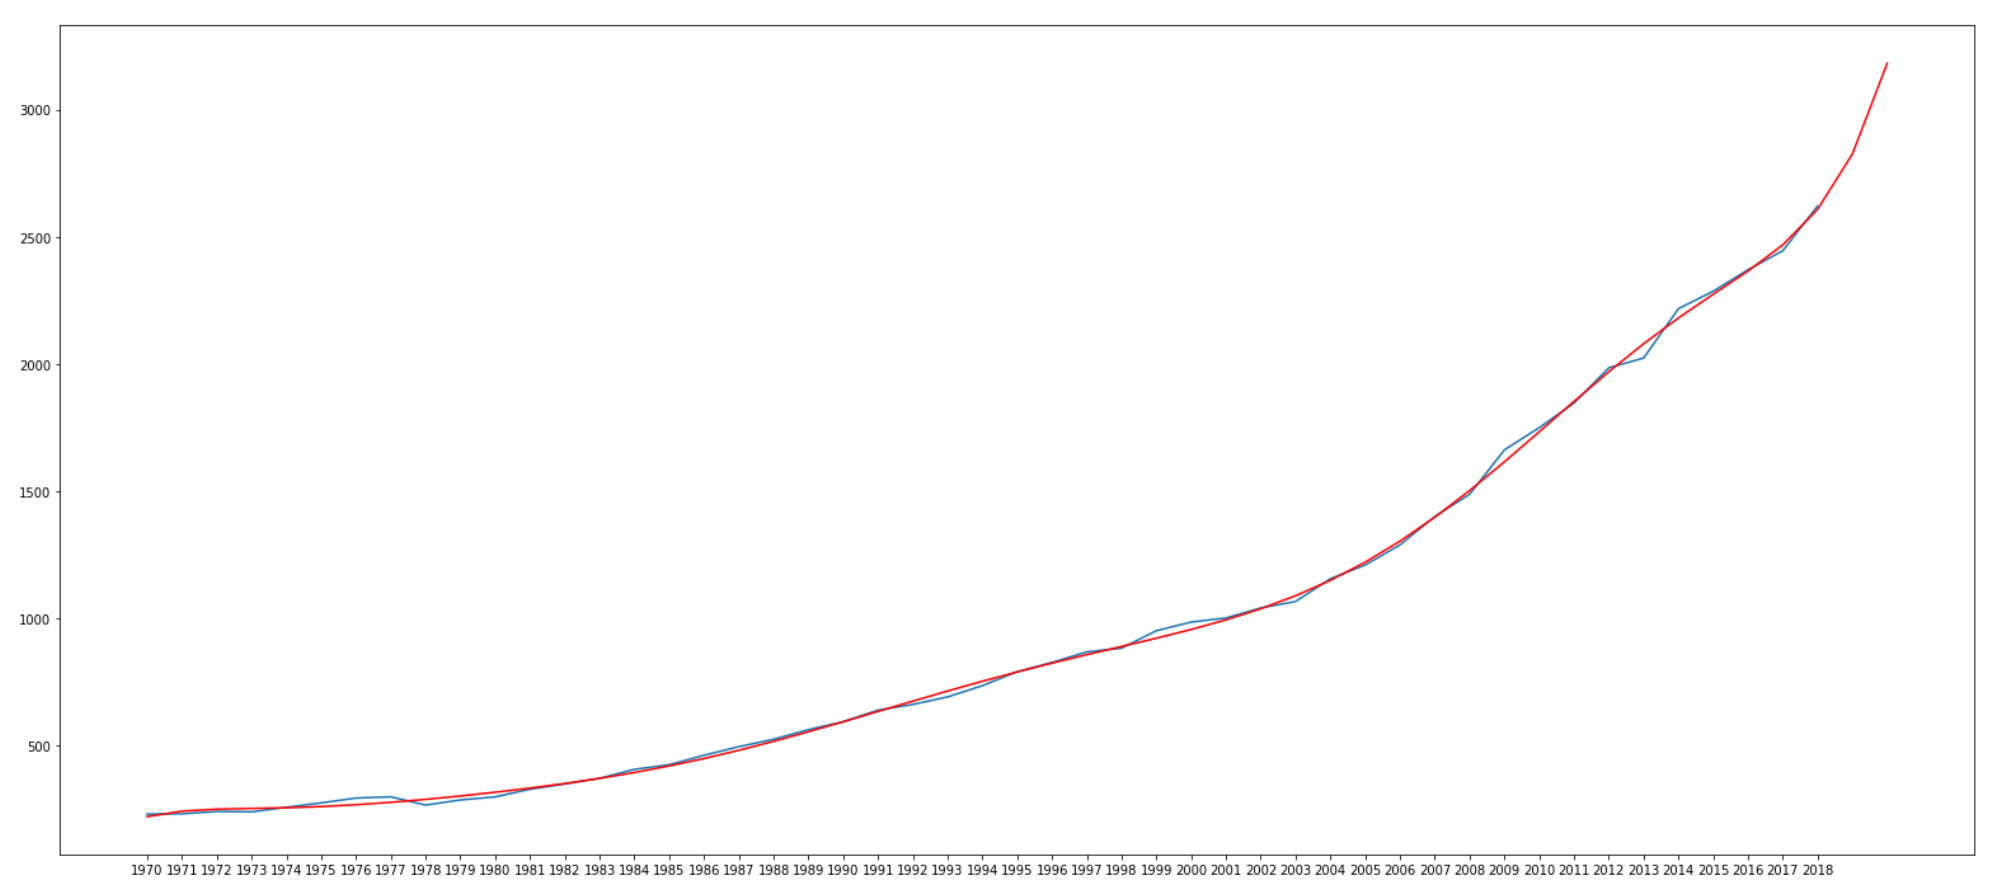
\includegraphics[width=0.5\linewidth]{ziedPNGS/7}}
	\caption{These graphs present the predicted emissions.}
	\label{fig:Results}
\end{figure}

\subsection{Sector indicators}

Knowing each sectors usual contribution to the total emissions for each country, we want to find the behavior of the \co emissions of each sector during the lock-down. To do so, we use monthly data available to us that can be seen as an indicator for the respective sector. For each country, we extract one value per month in 2020 that we apply to our estimated 2020 \co emission data without considering COVID-19. In conclusion, we modulate our yearly data with monthly values to obtain monthly \co emission data for 2020.

\textbf{Power Industry}
Indicators:
{Natural gas prices:} \cite{gas}, {Brent spot prices:} \cite{brent}, {Electricity, gas, steam and air conditioning supply:} \cite{production}, 
{Supply oil:} \cite{production}.

Strategy:
\begin{enumerate}
	\item \textbf{Selection of most correlated indicator:} we looked for only one indicator per country which could explain the behavior of the emissions. 
	\item \textbf{Time series prediction from december of 2019:} we predict the last months when the COVID-19 had not a big impact, in order to have a reference to compare. The prediction was using the SARIMA model \cite{sarima}. 
	\item \textbf{Extracting COVID-19 influence:} as we have current data from the last months (from January to May of 2020), we can observe a relative change respect the predicted values.
\end{enumerate}


\textbf{Buildings}
Indicators:
\begin{itemize}%todo: add citations to bibliography
	\item \textbf{Iron steel price.}
	Source: Federal reserve Bank of St. Louis
	\url{https://fred.stlouisfed.org/series/WPU101}
	\item \textbf{Producer Price index by industry: cement and concrete product manufacturing.}
	Source:  Federal reserve Bank of St. Louis
	\url{https://fred.stlouisfed.org/series/PCU32733273}
	\item \textbf{Industrial Production: Durable Goods: Cement and concrete products.}
	Source:  Federal reserve Bank of St. Louis
	\url{https://fred.stlouisfed.org/series/IPG3273S}
	\item \textbf{Total construction spending.}
	Source:  Federal reserve Bank of St. Louis
	\url{https://fred.stlouisfed.org/series/TTLCONS}
\end{itemize}%todo: Were they all used? Spelling, Reduce info
Strategy:
\begin{enumerate}
	\item \textbf{Model training:} For each country a support vector machine regression model was used, in order to allow the employment of different kernels. The eight selected regions (USA, EU, Brazil, Russia, Japan, China, India, Canada)  were fitted on 2004-2018 yearly \co emission data. To avoid overfitting, the validation loss was optimized on 30\% of the data by using a gridsearch method to evaluate the best degree of kernel regularization. 
	\item \textbf{Prediction:} Afterwards, the model was used to predict monthly data in 2020 with the same indicators.
	\item \textbf{Extracting COVID-19 influence:} To extract the information whether the emissions had gone down or not due to COVID-19, we compare the 2020 data with an interpolation of the global emissions up to 2018.
\end{enumerate}

\textbf{Mobility data}

\paragraph{Analysis of available datasets}

As already described in Milestone 2, we had four data sets suitable for this sector. These were two data sets on international flight activity and two mobility data sets from Google and Apple. The aviation data sets could not be used for this sector, as the number of flights was not stated explicitly for every country. We then decided to take a closer look at the Apple mobility data set, as it was easy to handle but still contained all necessary information. For every country, it contains \textit{walking} and \textit{driving} mobility data and wherever available, \textit{transit} mobility data as well. We had to pre-process this dataset a little by grouping the data of 26 out of 28 EU countries (Cyprus and Malta were not available). Furthermore, we applied a 7-day \textit{moving average} filter, to account for changes throughout the week. Unfortunately, we could not gather mobility data for China, as it was neither in the Apple mobility data set nor in the Google mobility data set. This can be directly attributed to China's restrictive handling of sensitive data. We also tried to gather information from \textit{Baidu Maps}, China's \textit{Google Maps} equivalent so-to-say. However, this proved to be very difficult, as the files are prepared in Chinese and nobody in our team is able to read Chinese. Therefore, we had to calculate China's mobility indicator from other countries' mobility data and do a few assumptions.

\paragraph{Data visualization}

As it is interesting to see the drop in international flights, we depicted it in \autoref{fig:flights}. In \autoref{fig:driving} and \ref{fig:transit}, we show the raw, unprocessed data and our result after applying a moving average filter. From the two figures, we can see that \textit{driving} mobility almost recovered to a normal level for most countries, while \textit{transit} mobility is still low for all countries except Japan.


\begin{figure}[hb!]
	\centering
	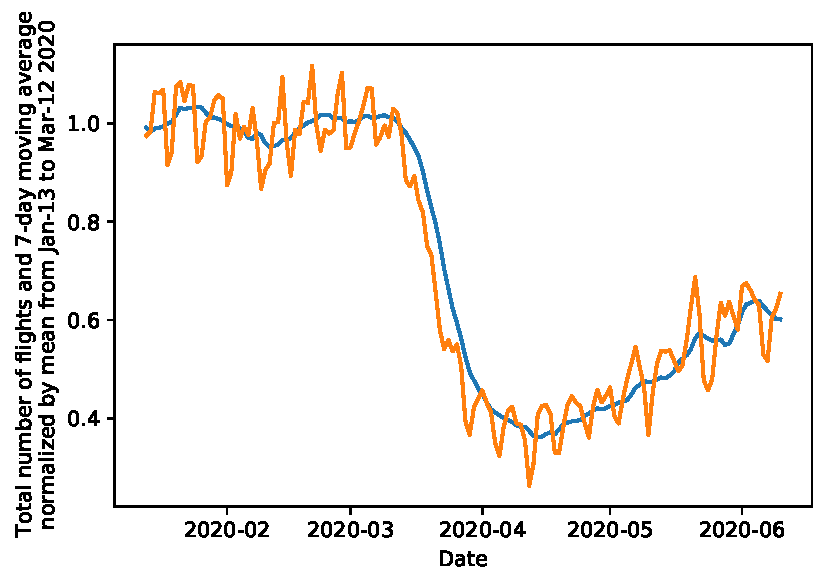
\includegraphics[width=0.7\linewidth]{../predictions/flights.pdf}
	\caption{International flights data.}
	\label{fig:flights}
\end{figure}


\begin{figure}[h!]
	\centering
	\subfloat[Raw driving data]{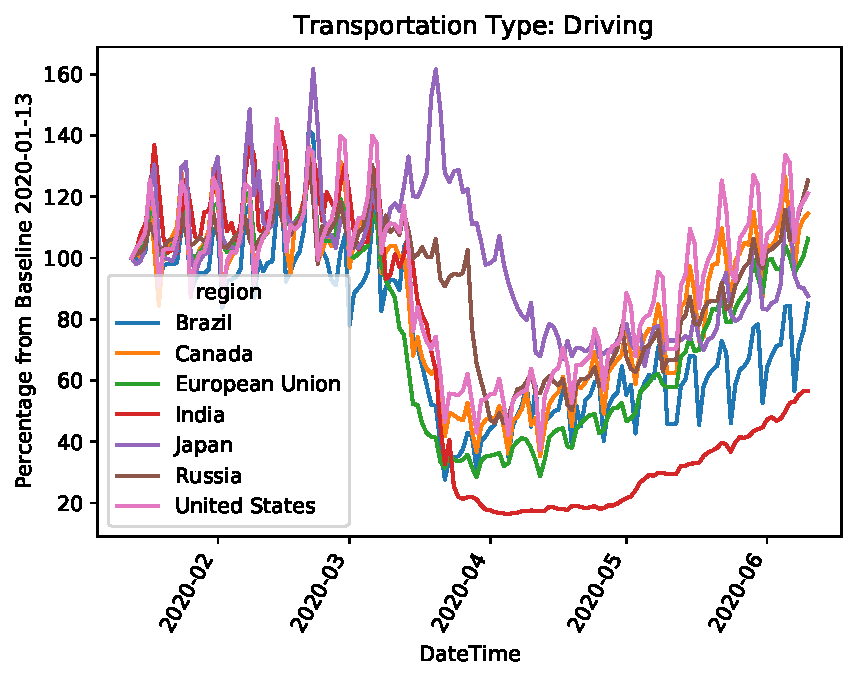
\includegraphics[width=0.48\linewidth]{../predictions/driving.pdf}}
	\hfill
	\subfloat[Driving data with moving average]{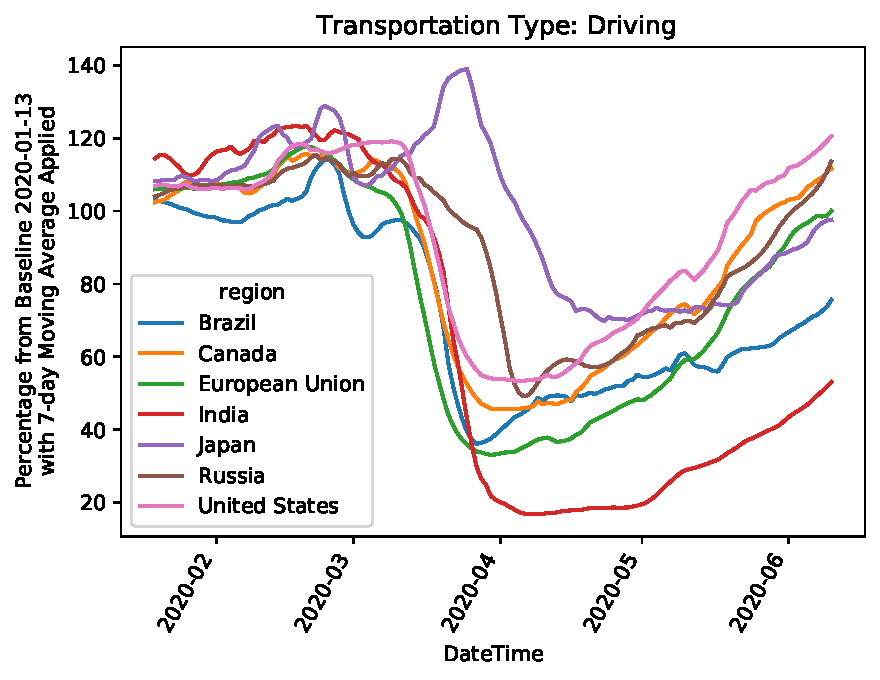
\includegraphics[width=0.48\linewidth]{../predictions/driving_ma.pdf}}
	\caption{Mobility data. A steep drop is visible for all countries.}
	\label{fig:driving}
\end{figure}

\begin{figure}[h!]
	\centering
	\subfloat[Raw transit data]{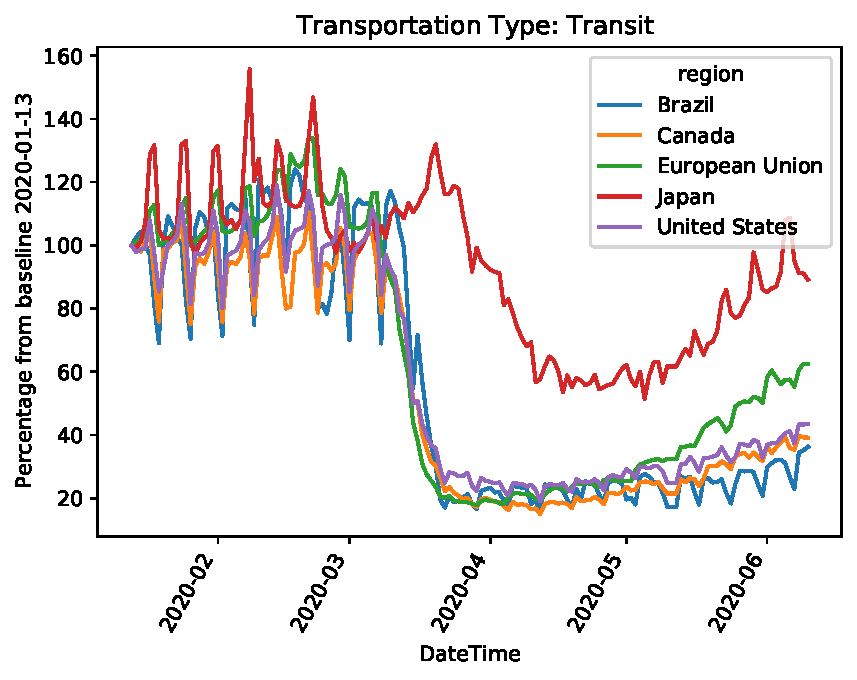
\includegraphics[width=0.48\linewidth]{../predictions/transit.pdf}}
	\hfill
	\subfloat[Transit data with moving average]{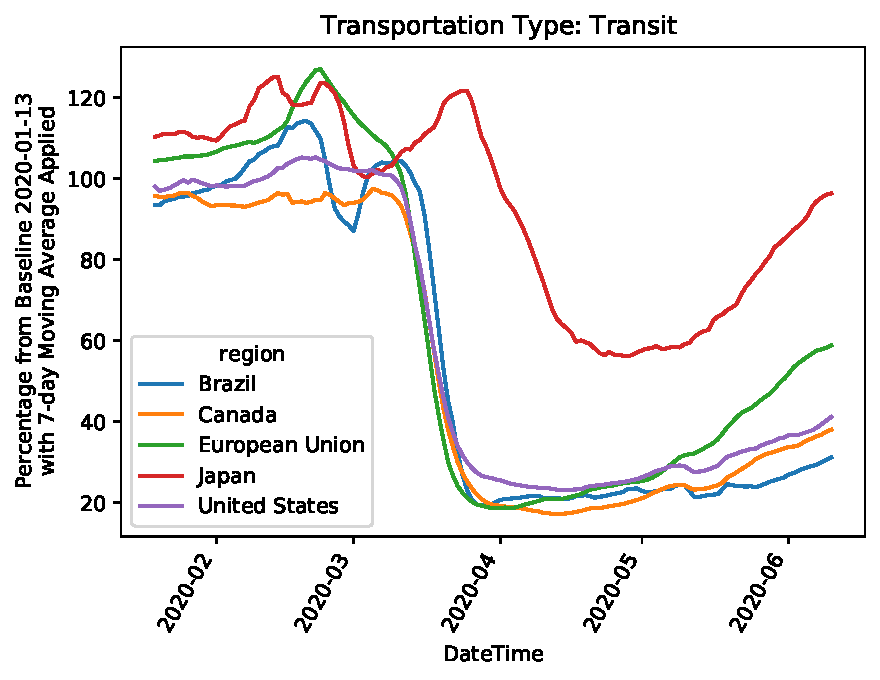
\includegraphics[width=0.48\linewidth]{../predictions/transit_ma.pdf}}
	\caption{Mobility data. A steep drop is visible for all countries that transit data was available for.}
	\label{fig:transit}
\end{figure}

\subsubsection{Other industries}

This sector is called \textit{other industries}, which one might misunderstand at the first glance. We wanted to be consistent with the sector distribution we found, where this sector is labeled other industry. Actually, it simply refers to all industry except \textit{power industry}.

\paragraph{Strategy}
After conducting some research on how to find suitable indicators for this sector, we found out that global steel production fits our needs. Monthly data is readily available and data researchers are able to predict a country's economic growth with it~\cite{Ravazzolo2020}.
Furthermore, \textit{Le Quéré et al.} model monthly \co data of the industry sector using US steel production data as well~\cite{LeQuere2020}.

\paragraph{Data}
We found recent data of worldwide steel production from January 2019 on, depicted in \autoref{fig:steelallcountries}.
For a longer period of time, we found US steel production data. As shown in \autoref{fig:steelUS}, it ranges from mid 2015 until mid 2020.
\begin{figure}[hbt]
	\centering
	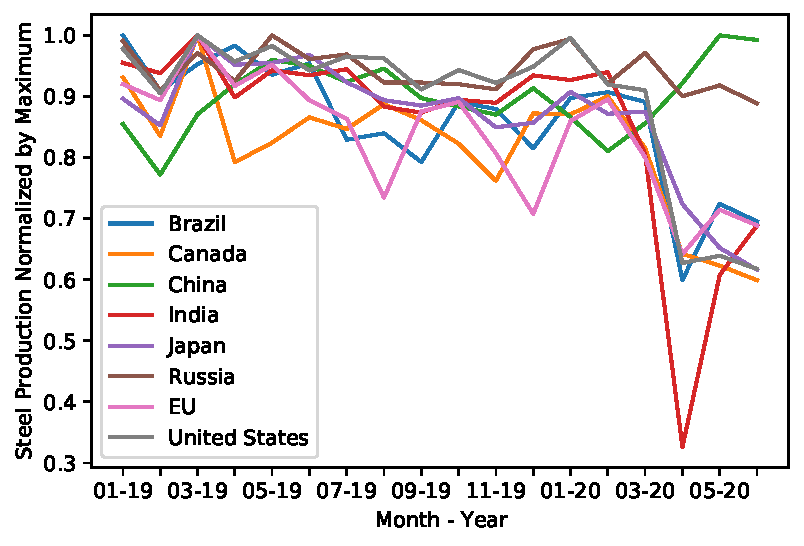
\includegraphics[width=0.69\linewidth]{../predictions/steelAllCountries.pdf}
	\caption{Steel output of all eight countries considered, normalized by the respective maximum for a better comparison.}
	\label{fig:steelallcountries}
\end{figure}

\begin{figure}[hbt]
	\centering
	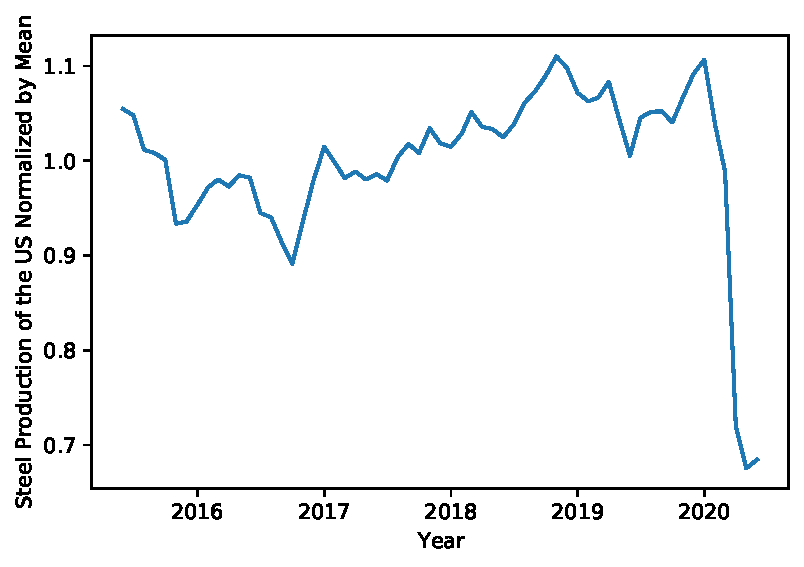
\includegraphics[width=0.69\linewidth]{../predictions/steelUS.pdf}
	\caption{Steel output of the US, normalized by the mean in the years 2015 to 2020.}
	\label{fig:steelUS}
\end{figure}

\newpage

\paragraph{Method}
In contrast to \textit{Le Quéré et al.}, we wanted to use each country's own steel production and not only US data. However, only recent data from 2019 until now is available for free for every country considered in this work. Obviously, one can not find seasonality trends from that. Thus, we use the recent data we have to find a preliminary indicator without seasonality adjustments for each country first, as depicted in \autoref{fig:otherindustry_notadjusted}. For this, we took the early 2020 data of this month and divided it by the early 2020 data and thus obtain a percentage of the steel production output in early 2020 compared to early 2019. 

We then use US steel production data to find a seasonality trend. Furthermore, we assume here that we can transfer this seasonality adjustment to all other countries as well. Our strategy to find a seasonality trend begins with finding mean values of steel production in a given year. We assume that these mean values centered on a given time-point, are the steel production values with seasonality removed. The ratio of the new value without the seasonality effect to the old value is the seasonality trend. Since we can calculate the trend for four different years by using the US data, and we do not want to overfit for a single year, we take the average of seasonality trends of 4 years. Seasonally adjusted steel output of the US can be seen in \autoref{fig:steelUS_adjusted}

\subsubsection{Other sectors}

The main sector which has a big impact on the \co emission considered such as \emph{other sectors} is agriculture. In 2018, it had an average contribution of 12.56\% to the worlds greenhouse gas emissions. In this section, we considered agriculture indicators which can have the most impact on the \co emission, such as rice and soybeans cultivation, and cattle farming. 

\paragraph{Indicators}

\subparagraph{Cattle farming}

Without any doubts, we can say that it is the livestock farming which has the greatest impact on \co emission in this sector. Cattle farming has a huge impact on the greenhouse gas emissions not only by breathing. The carbon balance of livestock farming includes emissions related to land-use changes, in particular the replacement of forests with pastures and arable fields for fodder production (i.e. deforestation). This means the elimination of huge carbon reservoirs, which are forests, and their replacement with much less capacious agricultural areas. It is estimated that as a result of deforestation, up to 2.4 billion tons of \co are emitted into the atmosphere per year. It is the largest item in the balance of not only \co emissions from animal farming, but also the total greenhouse gas emissions from agriculture sector.

We takes into account 8 selected regions (USA, EU, Brazil, Russia, Japan, China, India and Canada), where 4 of them are the biggest world's providers of cattle (Brazil, India, USA, China) to show the trends in the recent 7 years and compare it with the estimation for all 2020 year. Because the recent data is very hard to collect, we are not able to say how fulfilled is this estimation for now. 

\begin{figure}[hb]
	\centering
	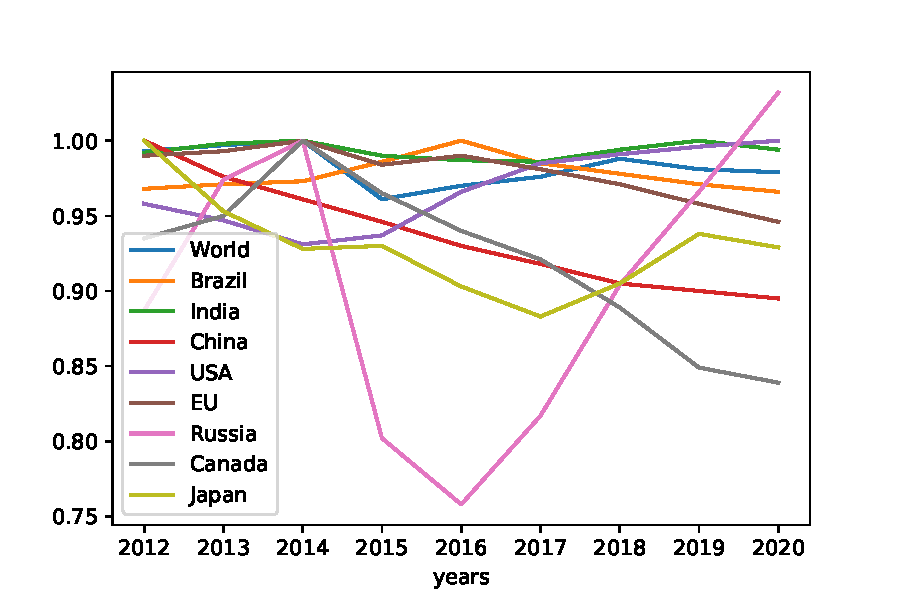
\includegraphics[width=0.7\linewidth]{../agriculture/Graph_cattle.pdf}
	\caption{Trends of cattle agriculture for 8 selected areas in seasons 2012-2019 with the estimation for all season 2020}
	\label{fig:Graph_cattle}
\end{figure}


\subparagraph{Plants: Analyzing rice and soybeans as indicators}

The greenhouse gas emissions profile for plant production differs significantly from that for sectors such as transport or industry. Emissions come from naturally variable biological processes that are numerous and complex, and management of these unavoidable emissions from biological processes is limited. Plant production naturally traps carbon in the soil and biomass during soil processes, also plants absorb \co from the atmosphere by photosynthesis. The emission results from the use of organic and inorganic fertilizers in the soil, as well as from the activity of microorganisms in the process of denitrification and nitrification. The potential to reduce the emissions of greenhouse gases from plant production gives the opportunity to combat global warming. 

We selected two plants which can have the biggest impact on greenhouse gas emission, soybean and rice. In case of rice, Canada is the most northerly rice production country and it has only one hectare crop of rice. That is why we decided to reject this country in our consideration in this sector. 

\begin{figure}
	\centering
	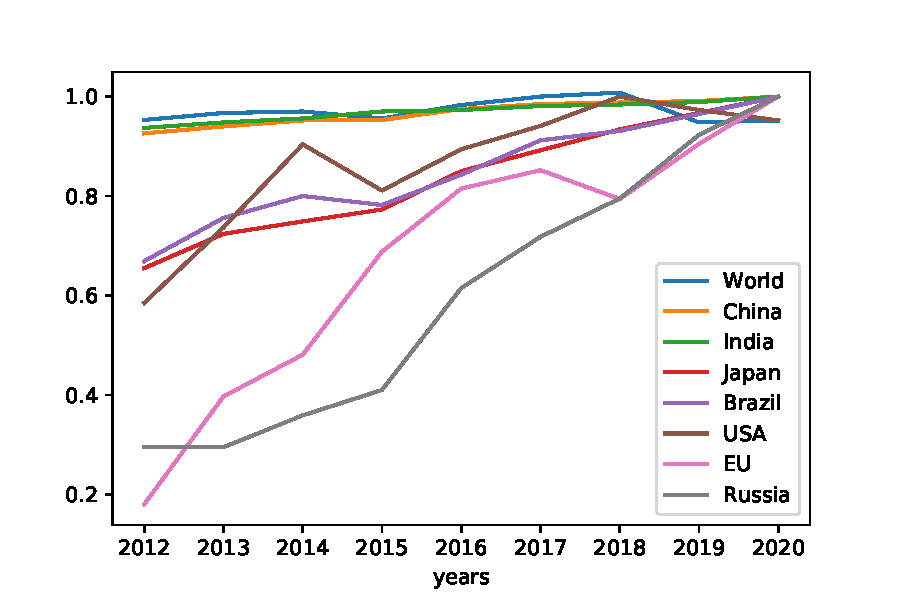
\includegraphics[width=0.7\linewidth]{../agriculture/Graph_rice.pdf}
	\caption{Trends of rice agriculture for 8 selected areas in seasons 2012-2019 with the estimation for all season 2020}
	\label{fig:Graph_rice}
\end{figure}

\begin{figure}
	\centering
	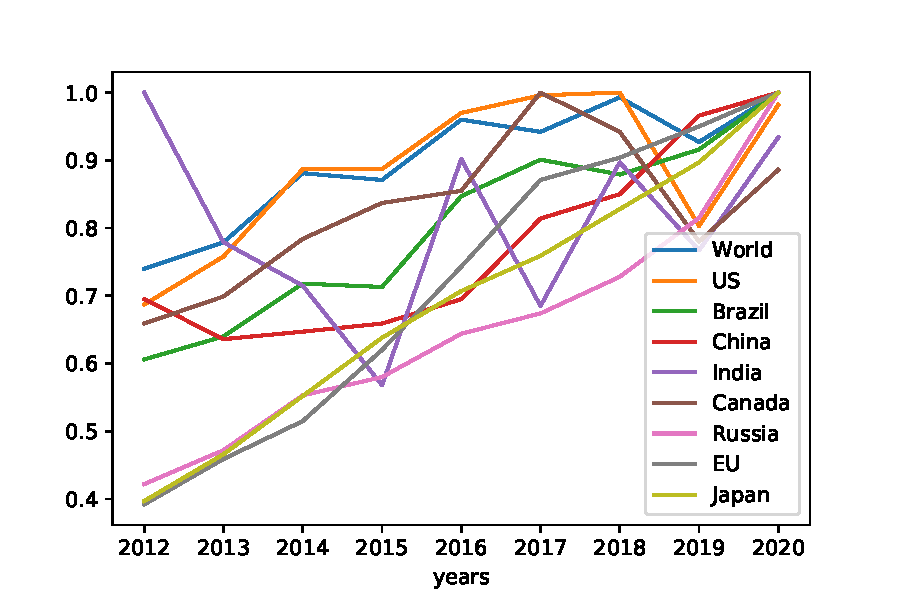
\includegraphics[width=0.7\linewidth]{../agriculture/Graph_soybean.pdf}
	\caption{Trends of soybean agriculture for 8 selected areas in seasons 2012-2019 with the estimation for all season 2020}
	\label{fig:Graph_soybean}
\end{figure}

We tried to gather detailed data on the processes that affect greenhouse gas emission from rice agriculture and their inter-relationships. It defines the shifting roles and potential future of these gases in causing global warming and the benefits and trade-offs of reducing emissions. It is known that when large amounts of organic matter are applied, the additional flux that is observed is due to both greater production and reduced emission. We noticed that rice cultivation is becoming less environmentally friendly in the face of a changing atmosphere. This is important because rice fields are one of the largest sources of methane and rice is the second most cultivated crop. Considering this issue with our project is to relate the \co emission and try to say how rising temperatures and the extra amount of carbon dioxide in the atmosphere affect rice crops and the amount of methane (CH\textsubscript{4}) released. It was figured out that the greater presence of \co resulted in increased methane emissions from rice fields, and in addition, high temperatures caused crops to decline. The methane in the rice fields is produced by microorganisms that absorb carbon dioxide. The more \co, the faster the rice grows, and the accelerated plant growth gives the microorganisms more energy. Rising \co levels will increase rice yields, but also the amount of methane. As a result, the amount of CH\textsubscript{4} emitted per kg of rice will increase. Rising temperatures have little effect on methane emissions, but as they reduce yields, the average amount of methane per kg of rice will increase. As a result, the higher \co concentration and higher temperatures projected at the end of the century may double the amount of methane per kg of rice produced. There are several options for reducing the amount of CH\textsubscript{4}, such as using alternative fertilizers and growing varieties that are less sensitive to heat.

Seeing that rice agriculture can have huge impact on the greenhouse gases emission, we try to show if there is any impact of COVID-19 pandemic on the rice production in the first half of the year, according to the estimation for the year 2020 and the seasonality of growing this crop. In the North China plains, the rice season is from May/June to August/September. In the Yangtze River Valley, rice is planted from April to June and harvested from August to October. In south-eastern China, the early (March to July) and late (June to November) rice crops are bountiful. So we can simplify that in all China there are two main seasons in the first half of the year and in the second half of the year. Taking India into account, the main rice growing season is June-July and it is harvested in November-December. The third world largest rice provider is Japan. In central Japan, it is from April–May to August–October. In southern Japan the rice season is from April -May to August–September. In Brazil the rice is planted from September to December and harvested from February through June, although later-planted rice grown in the northeast extends the season to August. In United States the harvest season in mid-September to October. 

\vfill

\begin{table}[h!]
	\centering
	\begin{tabular}{c c} 
		\hline
		Country & Season\\ 
		\hline\hline
		China & March to July and June to November \\ 
		India & November to December  \\
		Japan & April-May to August-October \\
		Brazil & February to June \\
		USA &  mid-September to October \\ 
		\hline
		&\\
	\end{tabular}
	\caption{Simplification of main seasonality periods of rice harvesting for 5 selected areas.}
	\label{tab:Seasonality_rice}
\end{table}

Next, we consider another one of a second biggest agriculture crop, soybean. The increase in soybean production as a source of protein and oil is being stimulated by the growing demand for livestock feed, food and numerous other applications. Significant greenhouse gas emissions can result from land use change due to the expansion and cultivation of soybean. However, this is complex to assess and the results can vary widely. The main point shows the importance of land use change in soybean greenhouse emissions, but significant differences were observed for the alternative scenarios, namely 0.1-17.8 kg \co per 1kg of soybean. The original land choice is a critical issue in ensuring the lowest soybean greenhouse balance and degraded grassland should preferably be used for soybean cultivation. The highest emissions occurs for tropical moist regions when rain forest is converted into soybean plantations. When land use change is not considered, the greenhouse gas emission intensity varies from 0.3 to 0.6 kg \co per 1 kg of soybean. It was calculated that all systems in tropical regions have higher greenhouse gas emissions than the others. It is also known, that N\textsubscript{2}O emissions play a major role in the greenhouse gas emissions from cultivation, although N\textsubscript{2}O emission calculations are very sensitive to the parameters and emission factors adopted.
If it comes to seasonality of soybean agriculture, the most of world soybean is harvested between March and the end of July (even in Brazil). In some tropical regions it can occur also during the winter season from November to December, but the amount does not have big impact for the world's production.